%! Author = Filippo Vissani
%! Date = 08/02/24
% !TeX root = ../thesis-main.tex

%----------------------------------------------------------------------------------------
\chapter{Design}
\label{chap:design}
%----------------------------------------------------------------------------------------

\section{Architecture}

As mentioned in \Cref{subsection:collektive-architecture}, Collektive consists of three main modules: \texttt{dsl}, \texttt{compiler-plugin} and \texttt{alchemist-incarnation-collektive}. \texttt{alchemist-incarnation-collektive} is responsible for enabling the integration of Collektive simulations into Alchemist. The \texttt{compiler-plugin} takes care of visiting the abstract syntax tree of the aggregate expression and modifying the function call stack to correctly align the devices that execute the aggregate program. The \texttt{dsl} module defines the following components:
\begin{itemize}
    \item \texttt{aggregate}: deals with defining the context related to a device, the semantics of aggregate constructs, and the data structures necessary for path definition and device alignment;
    \item \texttt{field}: Contains the definition of computational field and the related functionalities for manipulating the latter;
    \item \texttt{state}: defines the association between the paths and the results of their evaluations;
    \item \texttt{path}: Defines the data structures necessary to represent the abstract syntax tree relating to the aggregate expression;
    \item \texttt{networking}: defines the data structures necessary for distributed device communication.
\end{itemize}

Given the solutions proposed in \Cref{subsection:integration-solutions-identified}, in both cases, it is necessary to review some of the entities present in Collektive so that it is possible to detect and react to their changes. Regardless of the detailed solution chosen, given that the Collektive design allows it, it is possible to introduce the necessary functionalities as an extension of the current ones. The proposed architecture is shown in \Cref{fig:collektive-prm-architecture}, the components in gray are part of the current Collektive architecture, and those in orange introduce the entities that enable reactive aggregate programming. The component \texttt{reactive} extends \texttt{aggregate} to introduce a reactive version of the entities described above and \texttt{network} to allow reactive distributed communication between devices. The component \texttt{flow.extensions} is used to simplify some operations for combining and mapping flows. According to this design choice, the other modules in the project (\texttt{compiler-plugin} and \texttt{alchemist-incarnation-collektive}) are not altered; consequently, the reactive model introduced continues to make use of the compiler plugin for the definition of the paths.

\begin{figure}
    \centering
    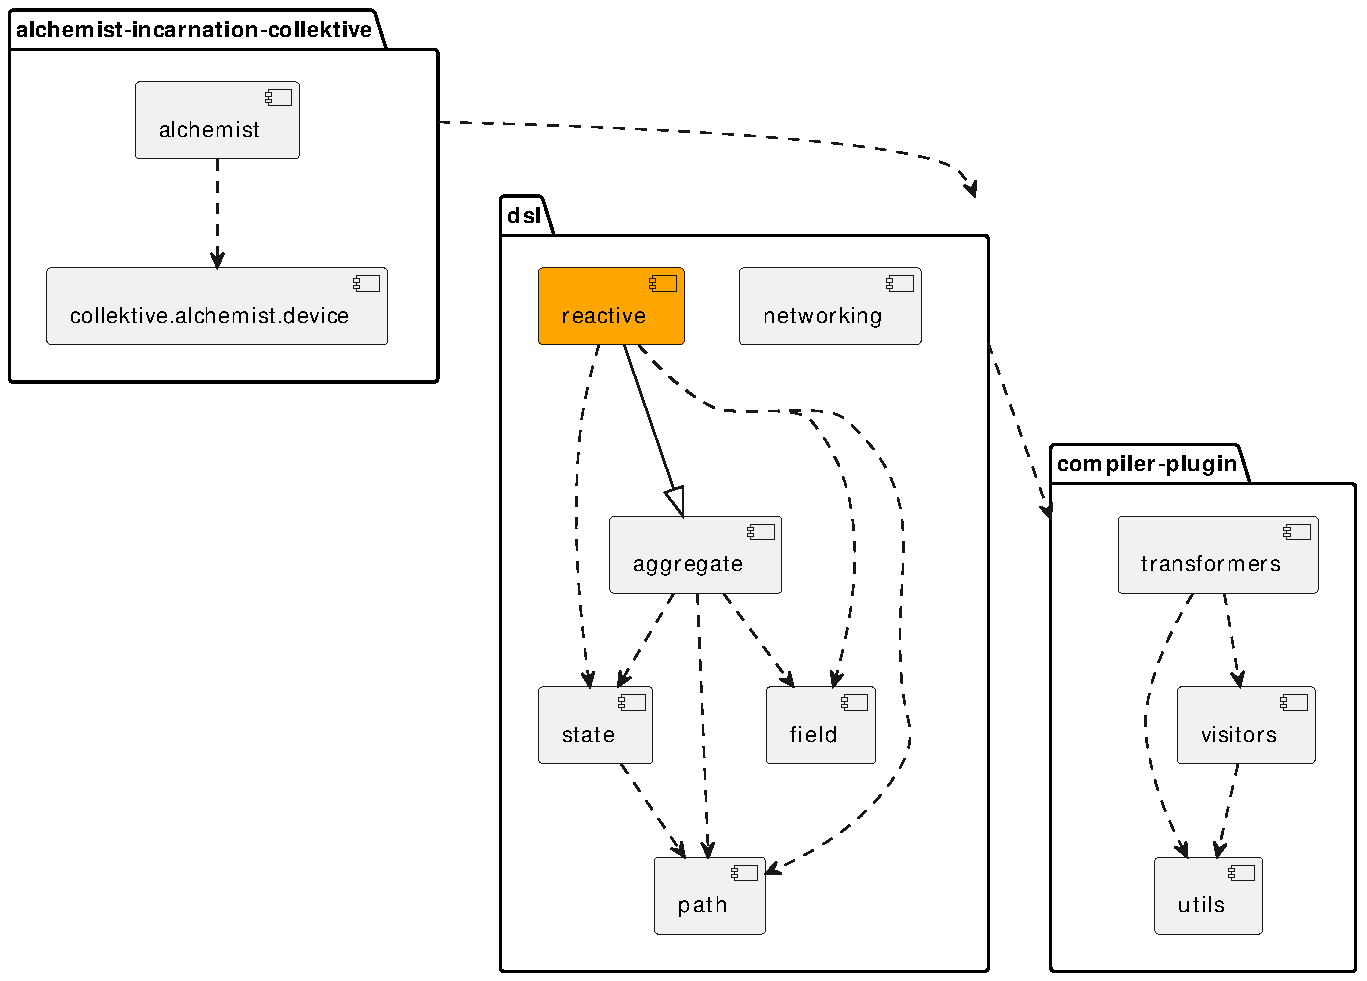
\includegraphics[width=\linewidth]{figures/collektive-prm-architecture.pdf}
    \caption{Architecture of the reactive model proposed. The gray-colored components are part of the original Collektive architecture, while the orange-colored components are used to introduce the reactive paradigm.}
    \label{fig:collektive-prm-architecture}
\end{figure}

\section{Detailed Design}

\subsection{Purely Reactive Model}
\label{subsection:purely-reactive-model}

The detailed design of the purely reactive model is shown in \Cref{fig:collektive-prm-design}. The class \texttt{RCollektive} contains the methods necessary for the execution of aggregate programs. Two new methods are added to this class which have \texttt{MutableStateFlow<List<InboundMessage<ID>>>} and \texttt{ReactiveNetwork<ID>} as parameters, respectively; this is because it is necessary to reevaluate the aggregate expression in whole or in part when new messages are received. Given that in this model the aggregate expression depends on values that change over time (neighbor messages and sensor status), the concept of expression result is also revised, so that it is reactive (\texttt{RAggregateResult}). The \texttt{Aggregate} interface takes care of defining the reactive versions of the aggregate constructs, the parameters of which are bound to \texttt{StateFlow} so that it is possible to reevaluate the constructs when the result of one of the functions they take as input changes. The \texttt{RAggregateContext} class extends \texttt{Aggregate} and provides the actual implementation of the aggregate constructs, as well as containing the reactive data structures necessary for managing the outbound messages and the state. This class makes use of the \texttt{StateFlow} extensions (\texttt{StateFlowExtensions}), which are used to simplify the mapping and combining of hot flows. The data structures that model the fields, stack and paths are not changed from the original design. Since the dependencies of aggregate sub-expressions are modeled reactively in this design, when the result of a sub-expression changes, only the sub-expressions that depend on that sub-expression are reevaluated.

The behavioral characteristics of the proposed model are reported below:

\begin{itemize}
    \item Computations occur reactively only when something changes in the environment, to avoid wasteful resource usage;
    \item Each device avoids broadcasting a message that did not change since the last one, with the direct consequence that no further message exchange is required if a computation reaches a stable configuration;
    \item If a portion of the computation depends on data that did not change, it is not be re-evaluated.
\end{itemize}

\begin{figure}
    \centering
    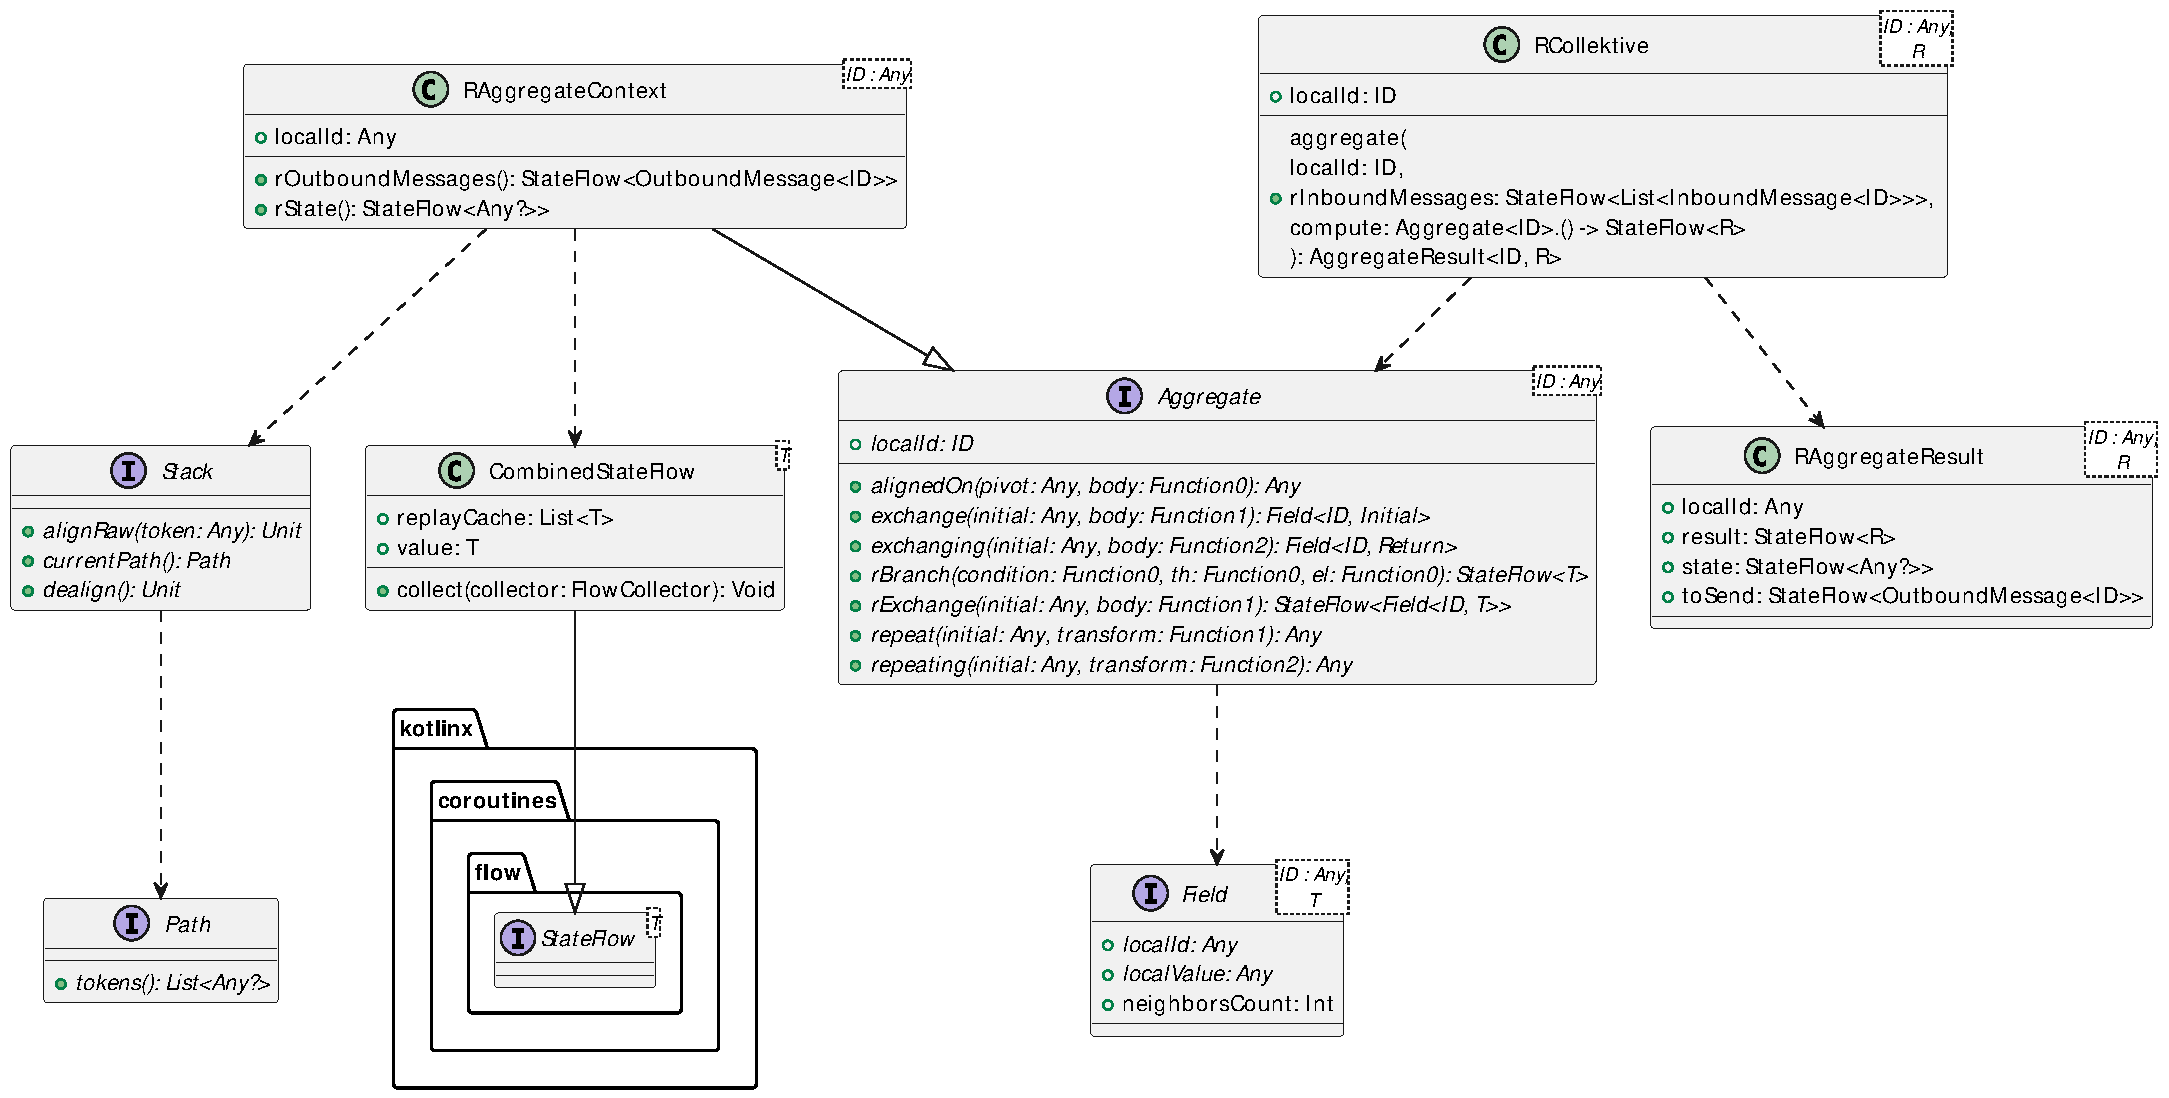
\includegraphics[width=\linewidth]{figures/collektive-prm-design.pdf}
    \caption{Detailed design of the purely reactive model proposed.}
    \label{fig:collektive-prm-design}
\end{figure}

\subsection{Model with Reactive Messages and Sensors}

The model with reactive messages and sensors, as defined by the name itself, simply introduces a reactive version of the messages received from neighbors and the state of the sensors. This implies that the changes made to the original Collektive design are more minimal than those of the model described in \Cref{subsection:purely-reactive-model}. The design of this model is described in \Cref{fig:collektive-rmsm-design}. Just like in the purely reactive model, the Collektive class implements two new versions of the \texttt{Aggregate} method, so it can receive messages via a \texttt{StateFlow<Iterable<InboundMessage<ID>>>} or a \texttt{ReactiveNetwork<ID>}. Again, the result of the \texttt{Aggregate} method is modeled as \texttt{StateFlow<AggregateResult<ID, R>>}. What changes in this design, compared to that relating to the purely reactive model, is that the \texttt{Aggregate} method implements in its entirety the logic that serves to make the evaluation of the aggregate expression reactive; as a consequence, contrary to what happens in the purely reactive model, the \texttt{AggregateContext} class is not modified. This naturally means that, when a message is received from a neighbor, the aggregate expression is reevaluated entirely, i.e. a round is performed.

\begin{figure}
    \centering
    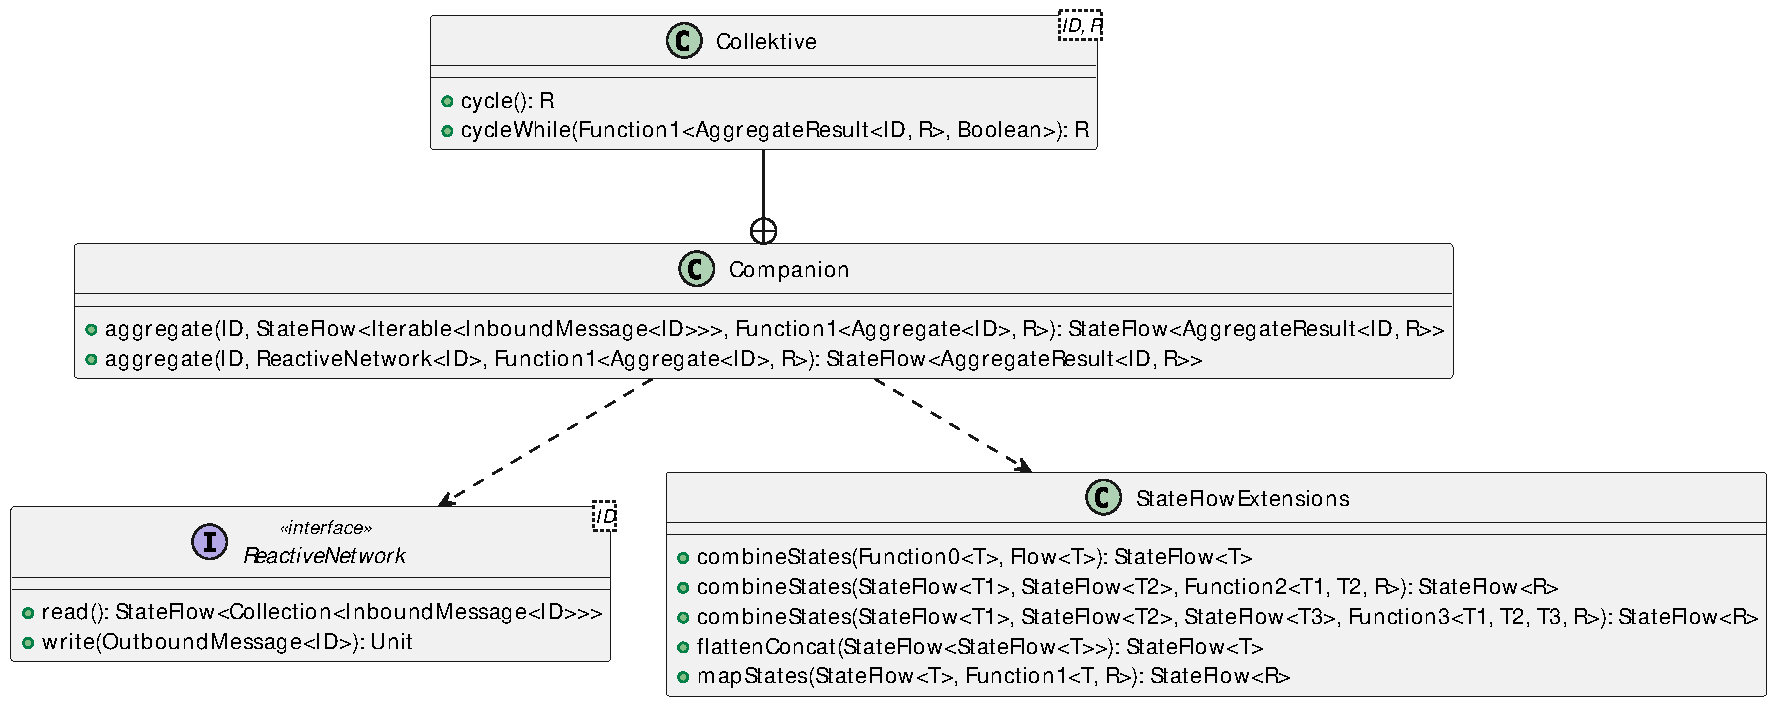
\includegraphics[width=\linewidth]{figures/collektive-rmsm-design.pdf}
    \caption{Detailed design of the model with reactive messages and sensors proposed.}
    \label{fig:collektive-rmsm-design}
\end{figure}
